\let\mymarginpar\marginpar

\documentclass[10pt,twoside]{article}

%\long\def\authornote#1{%
%        \leavevmode\unskip\raisebox{-3.5pt}{\rlap{$\scriptstyle\diamond$}}%
%        \marginpar{\raggedright\hbadness=10000
%        \def\baselinestretch{0.8}\tiny
%        \it #1\par}}
%\newcommand{\ville}[1]{\authornote{NOTE TO SELF: #1}}

\marginparwidth=1cm
\marginparsep=5pt
\newcommand\ville[1]{%
    \mymarginpar{\raggedright\hbadness=10000\tiny\it #1\par}}


\usepackage{amsmath} 
\usepackage{times}
\usepackage{amsmath,amsthm,amssymb}
\usepackage{fancyhdr}
\usepackage{moreverb}
\usepackage{graphicx}
\usepackage{amssymb}
\usepackage{url}
\usepackage{multirow} 
\usepackage[boxed, section]{algorithm}
%\usepackage{algorithm}
\usepackage{algorithmic}
\usepackage{cite}
\usepackage{multirow} 
\usepackage{rotating}
\usepackage{geometry}
\usepackage{fix-cm}
%\usepackage{subfigure}
\usepackage{natbib}
\usepackage{caption}
\usepackage{subcaption}

\renewcommand{\baselinestretch}{1.2}
\setlength{\topmargin}{-0.3in}
\setlength{\textwidth}{6in}
\setlength{\textheight}{8.5in}
\setlength{\oddsidemargin}{0.25in}
\setlength{\evensidemargin}{0.25in}
\raggedbottom




%\allowdisplaybreaks

% Math Macros.  It would be better to use the AMS LaTeX package,
% including the Bbb fonts, but I'm showing how to get by with the most
% primitive version of LaTeX.  I follow the naming convention to begin
% user-defined macro and variable names with the prefix "my" to make it
% easier to distiguish user-defined macros from LaTeX commands.
%
\newcommand{\myN}{\hbox{N\hspace*{-.9em}I\hspace*{.4em}}}
\newcommand{\myZ}{\hbox{Z}^+}
\newcommand{\myR}{\hbox{R}}
\renewcommand{\P}{\mathbb{P}}
\newcommand{\E}{\mathbb{E}}
\newtheorem{defi}{Definition}
\newtheorem{theorem}{Theorem}[section]
\newtheorem{lemma}[theorem]{Observation}
\newtheorem{observation}[theorem]{Observation}
\DeclareMathOperator*{\argmax}{arg\,max}

\theoremstyle{definition}
\newtheorem{example}[theorem]{Example}


\newcommand{\myfunction}[3]
{${#1} : {#2} \rightarrow {#3}$ }

\newcommand{\myzrfunction}[1]
{\myfunction{#1}{{\myZ}}{{\myR}}}


\newcommand{\mysection}[1]
{\noindent {\bf {#1}}}

%%%%%% Begin document with header and title %%%%%%%%%

\begin{document}

\title{Partial Information Model with an Application to Probability Extremization}
%\title{A Novel Framework for Analyzing Subjective Response Data}
\author{
Ville A. Satop\"a\"a, Robin Pemantle, and Lyle H. Ungar\\
\\
 \small Department of Statistics\\
 \small The Wharton School of the University of Pennsylvania\\
 \small Philadelphia, PA 19104- 6340, USA\\ [-0.25in]} \date{}
\maketitle

\pagestyle{myheadings}
\markboth{Partial Information Model}{Satop\"a\"a et al.}
\thispagestyle{empty}

\begin{abstract}
Randomness in scientific estimation is generally assumed to arise from
unmeasured or uncontrolled factors. However, when combining subjective probability estimates, heterogeneity
stemming from people's cognitive or information diversity is often
more important than measurement noise.  This paper presents a novel
framework that models the heterogeneity arising
from experts that use partially overlapping information sources, and applies that model to the task of
aggregating the probabilities given by a group of experts who forecast
whether an event will occur or not. Our model describes the
distribution of information across experts in terms of easily
interpretable parameters and shows how the optimal amount
of \textit{extremizing} of the average probability forecast (shifting
it closer to its nearest extreme) varies as a function of the experts'
information overlap.  Our model thus gives a more principled
understanding of the historically {\it ad hoc} practice of extremizing
average forecasts.
\end{abstract}

%data generative process. 


\section{Introduction}

Consulting experts are often asked to report their beliefs on various estimation problems. If the experts form their beliefs independently of each
other, their estimates are likely to be different. To analyze these
estimates with statistical methodology, it is mathematically
convenient to assume that any estimate heterogeneity arises
from a probability distribution. Under the most widely-used model, known as the \textit{classical measurement error model}, each estimate is assumed to be equal to the true value, i.e. signal plus some random error, i.e. noise. As the distribution of the error term is typically assumed to have mean zero, averaging the experts' estimates is expected to cancel out a part of the noise and hence lead to an accurate estimate of the true value. To illustrate this framework, consider a group of park rangers whose task is to measure the length of a mountain trail. Each of the rangers walks through the trail, assesses the length, and reports a personal estimate of the total length. Some of their estimates will be higher while some will be lower than the true length of the trail. Under the classical measurement error model these discrepancies follow a common distribution with mean zero and the average estimate gives an unbiased estimate of the trail length. It is important to notice that the classical measurement error model considers each estimate to have the same amount of signal. Therefore each expert is assumed to have the same information about the target estimation problem. Even though this seems appropriate for passive recording of measurements made by imprecise instruments, assuming constant signal and information among consulting experts is hardly reasonable. 


In many real-world problems and particularly in the social sciences the target quantity is not directly observable. Therefore data collection typically relies on polling of people. As each person has a different set of knowledge, the polled estimates cannot be assumed to have been generated under the same amount of information. If the signal varies among the estimates, any procedure that is used to aggregate them must take this heterogeneity into account. For instance, assume that each park ranger observes a different segment of the trail. Their information sets are therefore completely disjoint. Suppose that each ranger reports the length of the observed segment as the estimated length of the full trail. Modeling the estimates with the classical measurement error and hence averaging their estimates would dramatically underestimate the length of the trail. Summing the estimates, on other hand, gives an unbiased estimator of the trail length. If, however, some of the segments are not completely disjoint but overlap partially, the aggregation procedure must down-weight the overlapping segments to avoid potential double counting.  In this case the aggregator is a compromise between averaging and voting. Even though this example is clearly very simplistic, it illustrates that different information structures require different aggregators.  Only the extremes, namely averaging and summing (a.k.a. \textit{voting}), have been examined closely in previous literature. Most problems in the real world, however, involve partially overlapping information sets. Therefore studying the entire spectrum of aggregators is of outmost importance. 

The first contribution of this paper is to introduce a \textit{partial information model} that serves as an alternative to the classical measurement error model. The partial information model is particularly appropriate for analyzing the aforementioned spectrum of aggregators because it is based on the distribution of information among the experts. This distribution is characterized by the amount of information known by each expert and the amount information shared among the experts. For instance, consider two experts $A$ and $B$ who observe 10\% and 5\%  of the full information, respectively. If their information sets overlap by 2.5\% of the full information, their estimates are assumed to be positively correlated. Under the partial information model experts are assumed to give optimal estimates conditional on their private information sets. Therefore estimate heterogeneity does not stem from a probability distribution but  from differences in the experts' information sets. 

This must be contrasted with the \textit{interpreted signal framework} introduced by  \cite{hong2009interpreted}. Under their framework estimate heterogeneity stems from cognitive diversity instead of information diversity. An estimate is said to be ``interpreted" if the expert
first filters reality into a set of categories and then makes an
estimate by applying active cognitive effort to these categories. For
instance, consider a group of Olympic judges who are evaluating a figure skating
performance. Each judge first interprets the performance with the aid
of categories and then scrutinizes that experience into a final
score. As the set of categories is personal to each judge, it is left for the expert's judgment to decide how the world should be interpreted. This cognitive diversity is considered sufficient to explain any estimate heterogeneity. Even though the interpreted signal framework offers a highly realistic platform for modeling human response data, any previous work that is based on this framework has only produced abstract concepts and still lacks a formal model with quantitative predictions. The main problem is that it is not clear how ``cognitive diversity" can be measured in complex real-world situations. The amount of information known by an expert, on other hand, can be measured in practice. Therefore the partial information model offers a practically more relevant alternative that strikes a good balance between psychological realism and analytical convenience. 



%The experts are assumed to give optimal estimates conditional on their private information sets. This means that a larger information set typically leads to a more accurate estimate, and two identical information sets lead to the same estimate. In reality experts, however, do not typically make optimal use of their information. Therefore the partial information framework is a simplification of the real world. It is, however, a compromise that strikes a good balance between psychological realism and analytical convenience. 

%
%For instance, consider a group of
%experts who aim to eyeball the height of a building. Their estimates
%can be modeled as independent draws from a Gaussian distribution that
%is centered at the true height. This framework, which generally views data as consisting of signal plus noise,
%has been called the \textit{generated signal framework}  \cite{hong2009interpreted}. Even though distributional
%assumptions clearly oversimplify the reality, they are typically
%useful enough to improve our understanding of the world.
%
%
%Unfortunately, this is unlikely to be the case with subjective
%probability forecasts. \cite{hong2009interpreted} explain how standard
%distributional assumptions can be dramatically misaligned with the
%process that generates subjective responses. As an alternative to the
%generated signal framwork, they introduce the \textit{interpreted
%signal framework}. An estimate is said to be 'interpreted' if the expert
%first filters reality into set of categories and then makes an
%estimate by applying active cognitive effort to these categories. For
%instance, consider an Olympic judge who is evaluating a figure skating
%performance. The judge first interprets the performance with the aid
%of categories, and then scrutinizes that experience into a final
%score. Therefore any differences between estimates is assumed to arise
%from cognitive diversity instead of an underlying probability
%distribution. The interpreted signal framework is potentially  a more realistic modeling choice
%for subjective probability forecasts. Given that such data is
%common in real-world applications, such as product reviews,
%online auctions, and voting, this framework shows great potential in
%improving our understanding of many experimental
%results. Unfortunately, previous work  on using the interpreted signal framework has only produced
%abstract concept, and lacks formal models with quantitative predictions.

%LHU: we are focussing more on information diversity rather than cognitive diversity; I think this could be better brought out.



The second contribution of this paper is to apply the partial information model to probability aggregation. Combining multiple probability forecasts is an important problem with many applications including medical diagnosis (\citet{wilson1998prediction, pepe2003statistical}), political and socio-economic foresight (\citet{tetlock2005expert}), and meteorology (\citet{sanders1963subjective, vislocky1995improved, baars2005performance}). There is strong empirical evidence that bringing together the strengths of different experts by combining their probability forecasts into a single consensus, known as the \textit{crowd belief},  improves predictive performance. For instance, consider the aforementioned experts $A$ and $B$. The union of their information sets covers 12.5\% of the full information. Therefore it seems plausible that some combination of their probability forecasts is more informed than either one of the individual probabilities. The naive approach is to simply average the individual forecasts. To see why this approach can be problematic, recall that $A$'s forecast is based on a larger information set and hence typically more accurate than $B$'s forecast. Therefore $A$'s forecast is on average closer to the actual outcome of the event ($0$ if it does not happen and $1$ if it does happen) and should be given a higher weight in the final aggregate.  The average forecast, however, gives each forecast equal weight and hence ends up being necessarily too close to 0.5. Recent developments suggest that shifting the average probability closer to its nearest extreme (0.0 or 1.0), known as \textit{extremizing}, yields improved forecasting performance. For instance, \citet{satopaa} use a linear regression model in the logit-space to derive an extremizing aggregator that performs well on real-world data. \citet{Ranjan08} propose transforming the average probability with the cumulative distribution function (CDF) of a beta distribution. If both the shape and scale of this beta distribution are equal and constrained to be at least 1.0,  the aggregator extremizes and has some attractive theoretical properties (\cite{Wallsten2001}).  \citet{Baron} provide yet another extremizing aggregator in addition to two intuitive justifications for extremizing.


These aggregators, however, are based on \textit{ad hoc} techniques that learn the amount of extremization by optimizing a scoring rule over a separate training set (for a discussion on scoring rules see \citet{Gneiting04strictlyproper}). It is concerning that extremization does not arise naturally from the underlying model. These aggregators are also too detached from the psychology literature to provide any insight beyond the aggregate probability. Therefore it is still not well-understood when and how much the average probability should be extremized. This paper remedies these shortcomings by developing an aggregator that is based on the partial information model. The resulting aggregator depends on the distribution of information among the experts and can be used to study an entire spectrum of probability aggregators. Therefore it can be used for learning about the class of information structures that make any particular procedure, such as averaging or voting, work well in practice. The aggregator also provides a closed-form expression for the amount of extremizing that the should be performed for the average probit-forecast. Under a simplified information structure this expressions depends only on three intuitive parameters. This allows us to visualize extremization and make concrete statements on when and how much extremization should be performed. 




The first section of this paper introduces our partial information model and illustrates  it on probability forecasts made by a group of expert on events with two potential outcomes. The second section derives a closed-form expression for the amount of extremization and analyzes it under unstructured, disjoint, and compound symmetric information structures. The third section provides an extension to events with more than two potential outcomes. After this the paper concludes with a discussion of  model limitations and future directions. 



%\section{Information Theoretic Framework}
%This section discusses the partial information framework in comparison to the generated and interpreted signal frameworks. This comparison is by no means comprehensive as signal generation is a large part of the statistical literature. The first subsection builds  intuition via a simple example. The second subsection provides a technical comparison. 
%
%\subsection{Simple Example}
%Consider two experts $1$ and $2$ who are observing a hockey tournament. The tournament consists of three games played between teams RED and BLUE. After seeing the outcome of the first game, the experts are asked to report the probability of RED winning the tournament. Assume that RED wins if $G_1 + G_2 + G_3 \geq 0$, where $G_k \in \{-1,1\}$ indicates whether RED won the $k$th game. Suppose that all 8 possible combinations are equally likely. 
%%Therefore the true probability of team RED winning the tournament is 1/2.
%
%\begin{enumerate}
%\item[] \textit{Generated Estimate:} Based on the first game, the $i$th expert believes that RED has an independent chance of $q_i$ winning any of the two remaining games. The probability $q_i$ is assumed to arise from a probability distribution defined on the unit interval. Therefore any individual differences in the way the experts process the first game and turn the acquired information into probabilities $q_1$ and $q_2$ are assumed to stem from a probability distribution. The exports report
%\begin{align}
%p_i &= \begin{cases}
%q_i(2-q_i) & \text{ if } G_1 = 1\\
%q_i^2 & \text{ if } G_1 = -1
%\end{cases}
%\label{basisP}
%\end{align}
%
%\item[] \textit{Interpreted Estimate:} Interpretations are different ways of seeing the first game. Assume that RED's performance can be attributed entirely to its \textit{defense} $D$ and \textit{offense} $O$ that are equally likely to be either good $1$ or bad $-1$. Expert 1 follows only the defense and expert 2 looks only at the offensive play. Based on these attributes the experts construct their final predictive models. Under the generated signal framework the details of these predictive models are abstracted into a probability distribution. Under the interpreted signal framework, however, the details are fixed and known. For instance, the experts may report (\ref{basisP}) but with
%%If RED wins a game when $D + 2O \geq 2$, the experts report (\ref{basisP}) but with
%\begin{align*}
%q_1 = \begin{cases}
%2/3 & \text{ if } D = 1\\
%1/3 &  \text{ if } D = -1
%\end{cases}
%&& q_2 &= \begin{cases}
%3/5 & \text{ if } O = 1\\
%2/5 & \text{ if } O = -1
%\end{cases}
%\end{align*}
%Each expert interprets the available information independently and subjectively.  Therefore even if the experts observed the same attributes of the game, their probability forecasts do not need to be the same. 
%
%
%\item[] \textit{Information Theoretic Estimate:} The experts know that RED has a 1/2 chance of winning any given game. Suppose that expert 1 knows the number of wins in the first two games, i.e. the value of $G_1 + G_2$, but not necessarily the separate outcomes of the two games. Assume that expert 2 only knows the outcome of the first game $G_1$. Then,
%\begin{align*}
%p_1 = \begin{cases}
%0 & \text{ if } G_1 + G_2 = -2\\
%1/2 & \text{ if } G_1 + G_2 = 0\\
%1 & \text{ if } G_1 + G_2 = 2\\
%\end{cases}
%&& p_2 = \begin{cases}
%1/4 & \text{ if } G_1 = -1\\
%3/4 & \text{ if } G_1 = 1\\
%\end{cases}
%\end{align*}
%Experts 1 and 2 know 2/3 and 1/3 of the full information, respectively. Their predictive models are completely determined by the size of their private information sets. As their information sets overlap by 1/3 of the full information, their probability forecasts are positively correlated. In this example, the correlation coefficient for their forecasts is $\sqrt{2}/2$.  
%
%
%\end{enumerate}


%\section{Partial Information Framework}
%\subsection{Technical Details}
%Let  $(\Omega, \mathcal{F}, \P)$ be a probability space, where the set $\Omega$ contains all possible states of the world, the $\sigma$-field $\mathcal{F}$ consists of all subsets of $\Omega$, and $\P$ is a probability measure. Let $A \in \mathcal{F}$ denote an event of interest. 
%%The set of possible outcomes is denoted with $S$. For the sake of illustration, assume that  $S = \{G, B\}$, where $G$ and $B$ denote good and bad outcomes, respectively. The outcome function $F: \Omega \to S$ is a random variable that maps the state of the world to the true outcome. 
%The experts aim to forecast the probability $p = \P(A)$. Even though this paper focuses on probability estimates, the following discussion can be easily generalized to different types of estimates. 
%
%Generated estimates can be considered as noisy or distorted versions of $p$. In other words, if $\xi: [0,1] \to [0,1]$ is a noise function that randomly distorts a probability, then a generated probability forecasts is realized by $p_i = \xi(p)$. Due to its mathematical convenience, this framework is typically applied to subjective response data. Unfortunately, it can be drastically misaligned with the psychology literature and hence lead to results that are not reflective of the actual process that generates the estimates.
%
%%Therefore any heterogeneity in the estimates stems from randomness that is typically assumed to be caused by uncontrolled or unmeasured factors. 
%%Even though this framework is mathematically convenient, it can be drastically misaligned with the psychology literature and hence lead to results that are not reflective of the actual environment that produces the estimates.
%%The interoperation framework aims to correct these shortcomings by proposing a model that is more cognitive based. See \cite{hong2009interpreted} for the original introduction. 
%Under the interpreted signal framework, the set of states $\Omega$ is assume to be finite. The expert partitions $\Omega$ into non-overlapping subsets. This partition, know as the \textit{interpretation}, is denoted with $\Pi^i = \{\pi_1^i, \pi_2^i, \dots, \pi_{n_i}^i\}$, where $\bigcup_{j=1}^{n_i} \pi_j^i = \Omega$ and  $\pi_j^i \cap \pi_k^i = \emptyset$ for $j \neq k$. The expert can only associate a state $\omega \in \Omega$ with a set in his partition. Therefore his information is incomplete as long as not all the sets of his partition are singletons. To make probability forecasts, the expert specifies a map $\phi_i: \Omega \to [0, 1]$ that is measurable with respect to $\Pi^i$. 
%%Therefore any differences in estimates stem from cognitive diversity of the experts. 
%Unfortunately, \cite{hong2009interpreted} do not specify how the expert constructs the map $\phi_i$. It is also not clear how to the set of states $\Omega$ should be specified in real-world applications.  



%The partial information framework removes these intractable components and provides a model that can be applied in practice. It does not assume detailed knowledge of the expert interpretations nor pose any structure or cardinality restrictions on $\Omega$.  Each expert simply forecasts $p_i = \P\left(A | \mathcal{F}_i\right)$ based on a private information set $\mathcal{F}_i \subseteq \mathcal{F}$. 
%%If the set $\Omega$ is finite, the information set $\mathcal{F}_i$ can be considered equivalent to the $\sigma$-field generated by the interpretation $\Pi^i$. 
%If two experts $i$ and $j$ share information such that $\mathcal{F}_i \cap \mathcal{F}_j \neq \emptyset$, then the correlation of their forecasts $p_i$ and $p_j$ is positive and proportional to the overlap in their information sets. This means that, similarly to the interpreted signal framework, any heterogeneity in the estimates stems from cognitive diversity. As the details of the information set $\mathcal{F}_i$ cannot be known in practice, the information known by the $i$th expert is quantified as a fraction of the full information. 
%For instance, expert $i$ may know 15\% of the full information while expert $j$ knows only 8\% of the full information. If in addition we specify that their shared information is, say, 3\% of the full information, we have established an information structure for these  experts. 
%This leads to a compromise that is mathematically convenient and psychologically reasonable. 

%This is shown in following sections where the partial information framework is applied to probability forecasts and their aggregation. 

%NOT OPTIMAL FORECASTS. THE EXPERTS DO NOT KNOW THE WHOLE PROCESS.

\section{Partial Information Framework}

The main component of the partial information model is a process that determines the final outcome. This process must be defined such that the experts can observe only a part of the process without knowing the final outcome. The experts then make conditional predictions given their observations of the process. To make this more specific, let  $(\Omega, \mathcal{F}, \P)$ be a probability space where the set $\Omega$ contains all possible states of the world, the $\sigma$-field $\mathcal{F}$ consists of all subsets of $\Omega$, and $\P$ is a probability measure. Denote the event of interest with $A \in \mathcal{F}$. 
%The set of possible outcomes is denoted with $S$. For the sake of illustration, assume that  $S = \{G, B\}$, where $G$ and $B$ denote good and bad outcomes, respectively. The outcome function $F: \Omega \to S$ is a random variable that maps the state of the world to the true outcome. 
%Therefore the experts aim to forecast the probability $p = \P(A)$. 
%The partial information framework removes these intractable components and provides a model that can be applied in practice. It does not assume detailed knowledge of the expert interpretations nor pose any structure or cardinality restrictions on $\Omega$. 
 Each expert forecasts $p_j = \P\left(A | \mathcal{F}_j\right)$ based on a private information set $\mathcal{F}_j \subseteq \mathcal{F}$. 
%If the set $\Omega$ is finite, the information set $\mathcal{F}_i$ can be considered equivalent to the $\sigma$-field generated by the interpretation $\Pi^i$. 
%If two experts $i$ and $j$ share information such that $\mathcal{F}_i \cap \mathcal{F}_j \neq \emptyset$, then the correlation of their forecasts $p_i$ and $p_j$ is positive and proportional to the overlap in their information sets. 
Therefore any heterogeneity in the estimates stems from information diversity. As the details of the information set $\mathcal{F}_i$ cannot be known in practice, the information known by the $i$th expert is quantified as a fraction of the full information. It is important to note that even though this paper focuses on probability estimation, the general framework of the partial information model can be  generalized to different types of estimates. 

\subsection{Probability Forecasts}
\label{Model}


Consider two experts 1 and 2 who forecast the probability of the event $A$ happening. Assume that the event $A$ is determined by a pool of white noise, and that the experts 1 and 2 see respective $\delta_1$ and $\delta_2$ portions of this noise. These portions form their information sets. The overlap in these information sets is a fixed share $\rho$ of what is seen by either expert. To make this more precise, consider the aforementioned probability space $(\Omega, \mathcal{F}, \P)$. On this space, define a white noise process that is indexed by the unit interval $S = [0,1]$. A white noise process is a Gaussian process $\{ X_B \}$ indexed by Borel measurable subsets $B$. The unit interval is endowed with the uniform measure $\mu$. This gives the white noise process a covariance structure $\text{cov}(X_B, X_{B'}) = \mu(B \cap B') = |B \cap B'|$, i.e. the length of the intersection. The target event is defined as $A = \{ X_{S} > 0\}$. Let $I_1, I_2 \subseteq S$ be the information sets observed by experts 1 and 2, respectively. Then,
\begin{align*}
\mu(I_1) = |I_1| &= \delta_1\\
\mu(I_2) = |I_2| &= \delta_2\\
\mu(I_1 \cap I_2) =  |I_1 \cap I_2| &= \rho
\end{align*}


\begin{figure}[t]
\centering
	\hspace{0em}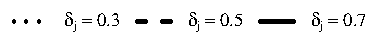
\includegraphics{LegendMarginal}

 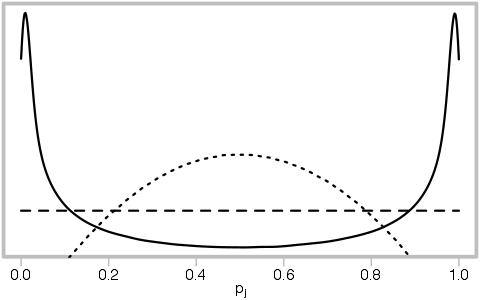
\includegraphics[width= 0.55\textwidth]{Marginals}
   \caption{The marginal distribution of $p_j$ under different levels of $\delta_j$. The more the expert knows, i.e. the higher $\delta_j$ is, the more the probability forecasts are concentrated around the extreme points 0 and 1.}
\label{marginals}
\end{figure}

The part of the process $X_{I_j}$ can be interpreted as the synthesis of the information known by expert $j$. Call $P_{I_j} = X_{I_j}/\sqrt{1-\delta_j}$ the probit forecast of the $j$th expert.  If $\Phi$ denotes the standard normal CDF, then the calibrated forecast given by the $j$th expert is
\begin{align*}
p_j &= \P\left(A | \mathcal{F}_{I_j}\right) = \Phi\left( P_{I_j}\right)
\end{align*}
Recall that if $Z$ is a standard normal random variable, then $\Phi(Z)$ is uniform on $[0,1]$. Therefore the marginal distribution of $p_j$ is uniform on $[0,1]$ when $\delta_j = 0.5$, i.e. when the expert knows half of the information. If the expert knows less than half of the information, i.e. $\delta_j < 0.5$, the marginal distribution of $p_j$ is unimodal at $0.5$ with the variance decreasing to 0 as $\delta_j \to 0$. On other hand, if the expert knows more than half of the information, i.e. $\delta_j > 0.5$, the marginal  distribution of $p_j$ is more heavily concentrated around extreme probabilities. In fact, when $\delta_j = 1$, the marginal distribution of $p_j$ is uniform over the set $\{0,1\}$. Figure \ref{marginals} illustrates these marginal distributions for $\delta_j$ equal to $0.3$, $0.5$, and $0.7$. 

\begin{figure}[htbp]
%   \hspace{-2em}
   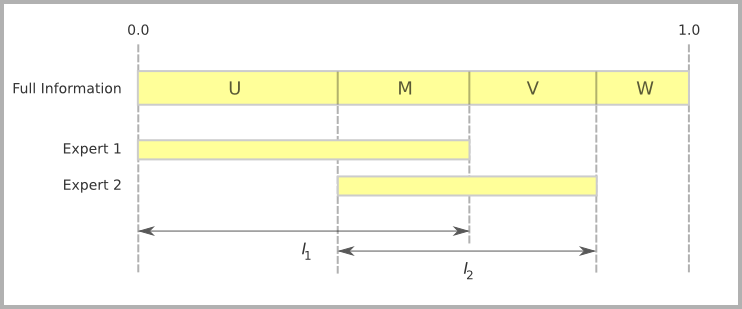
\includegraphics[width = \textwidth]{N=2} % requires the graphicx package
   \caption{Illustration of the partial information model with two experts.}
   \label{diagram2}
\end{figure}

It is helpful to begin the introduction of the model by first considering only two experts. Figure \ref{diagram2} illustrates this setup. The Gaussian process has been partitioned into four parts based on the experts' information sets $I_1$ and $I_2$:
\begin{align*}
 U &= X_{I_1 / I_2}
& M &= X_{I_1 \cap I_2}\\
 V &= X_{I_2 / I_1}
& W &= X_{(I_1 \cup I_2)^c}
\end{align*}
Then,
\begin{align*}
X_{I_1} &= U + M\\
X_{I_2} &= M + V\\
X_S &= U+M+V+W,
\end{align*}
where $U, V, M, W$ are independent Gaussians with respective variances $\delta_1-\rho$, $\delta_2-\rho$, $\rho$, $1+\rho-\delta_1 - \delta_2$. This gives $(X_{S}, X_{I_1}, X_{I_2})$ the following multivariate normal distribution. 
\begin{align}
\left(\begin{matrix} X_S \\ X_{I_1}\\ X_{I_2} \end{matrix}\right) &\sim \mathcal{N}\left(
 \boldsymbol{0},  \left(\begin{matrix} 
1 & \delta_1 & \delta_2\\
\delta_1 & \delta_1 &\rho\\
\delta_2 & \rho & \delta_2
 \end{matrix}\right)\right) \label{twoExperts}
\end{align}




\begin{figure}[htbp]
   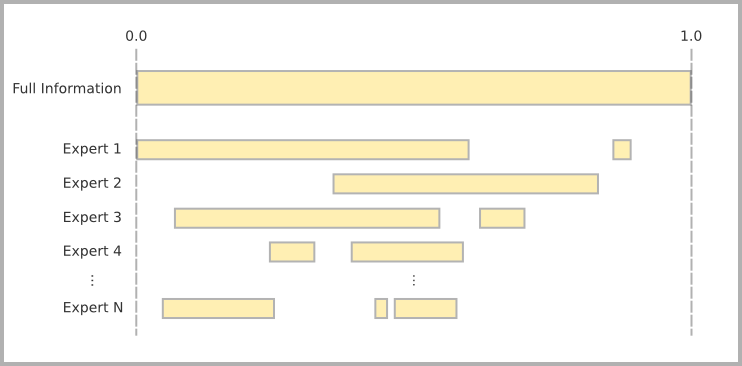
\includegraphics[width = \textwidth]{N=N} % requires the graphicx package
   \caption{Illustration of the partial information model with $N$ experts.}
   \label{diagramN}
\end{figure}



Consider now $N$ experts. Let $|I_j| = \delta_j$ be the amount of information known by the $j$th expert, and $|I_i \cap I_j| = \rho_{ij}$ be the information overlap between experts $i$ and $j$. Expression (\ref{twoExperts}) generalizes to the vector $(X_{S}, X_{I_1}, X_{I_2}, \dots, X_{I_N})$ as follows.
\begin{align}
\left(\begin{matrix} X_S \\ X_{I_1}\\ \vdots \\ X_{I_N} \end{matrix}\right) &\sim \mathcal{N}\left( \left(\begin{matrix} 
\mu_1 \\ \boldsymbol{\mu}_2
 \end{matrix}\right) =
 \boldsymbol{0}, \left(\begin{matrix} 
\Sigma_{11} & \Sigma_{12}\\
\Sigma_{21} & \Sigma_{22}\\
 \end{matrix}\right) 
 =
 \left(\begin{array}{c | c c cc }
1 & \delta_1 & \delta_2 & \dots & \delta_N  \\ \hline
\delta_1 & \delta_1 &\rho_{1,2} & \dots & \rho_{1,N}   \\ 
\delta_2 & \rho_{2,1} & \delta_2 & \dots & \rho_{2,N}  \\ 
\vdots & \vdots & \vdots & \ddots & \vdots  \\ 
\delta_N & \rho_{N,1} & \rho_{N,2} & \dots & \delta_N\\ 
 \end{array}\right)\right)  \label{NExperts}
\end{align}
This case is illustrated in Figure \ref{diagramN}. It is important to notice that $I_j$ does not have to be a contiguous segment of the unit interval. Instead, each expert can know any Borel measurable subset of the full information. The amount of information known by each expert and any potential overlap in these information sets is described in the sub-matrix $\Sigma_{22}$. Therefore each element in $\Sigma_{22}$ must be in the unit interval, and no off-diagonal element can be larger than the corresponding diagonal element in the same row. This matrix also has some technical conditions such as symmetry, non-singularity, and coherence. The matrix $\Sigma_{22}$ is coherent if and only if its information can be transformed into a diagram such as the one depicted by Figure \ref{diagramN}. 

%It is easy to show that all covariance matrices of size $N \times N$ are not coherent information structures. For instance, the off-diagonals of a covariance matrix  do not need to be upper bounded by its diagonal elements.  


%For instance, the matrix
%\begin{align*}
%\Sigma_{22} =  \left(\begin{array}{c c c}
%0.33 & 0.28 & 0.11\\
%0.28 & 0.33 & 0.25\\
%0.11 & 0.25 & 0.33\\
% \end{array}\right)
%\end{align*}
%is a valid covariance matrix but not a coherent information structure. The overlap $0.28$ between experts 1 and 2 is too large to allow for such a wide difference in their overlaps, $0.11$ and $0.25$ respectively, with the third expert's information set. 


%Thus $\bar{X}$ is extremized when
%\begin{align*}
% \frac{N \boldsymbol{1}_{N}' \Sigma_{22}^{-1} \boldsymbol{X}}{\boldsymbol{1}_{N}'  \boldsymbol{X}  \sqrt{N - \boldsymbol{1}_{N}' \Sigma_{22}^{-1} \boldsymbol{1}_{N}}}   &>& 1\\
% \frac{\boldsymbol{1}_{N}' \Sigma_{22}^{-1} \boldsymbol{X}}{\boldsymbol{1}_{N}'  \boldsymbol{X}  }   &>& \sqrt{ \frac{1}{N} - \frac{\boldsymbol{1}_{N}' \Sigma_{22}^{-1} \boldsymbol{1}_{N}}{N^2}},
%\end{align*}
%where the LHS side a weighed average of the elements of $\Sigma_{22}^{-1}$. This becomes clear after noticing that $\boldsymbol{X} / \boldsymbol{1}_{N}'  \boldsymbol{X}$ is a vector whose elements sum to 1. These give the weights for each respective column of $\Sigma_{22}^{-1}$. Hence the larger a given $X_j$ is the more influence it has in his weighted sum. The second term on RHS is the equally weighed average of $\Sigma_{22}^{-1}$. Notice that LHS increases as a function of $\Sigma_{22}^{-1}$ while RHS decreases. In addition, if $\boldsymbol{1}_{N}' \Sigma_{22}^{-1}  \boldsymbol{1}_{N} > \approx 1.1$ and fixed, then RHS decreases as $N$ increases. This largely revolves around understanding the interpretation of the precision matrix. 
%
%\begin{align*}
% \frac{( \boldsymbol{1}_{N}' \Sigma_{22}^{-1} \boldsymbol{X} )( \boldsymbol{X}'  \Sigma_{22}^{-1}\boldsymbol{1}_{N} )}{(\boldsymbol{1}_{N}'  \boldsymbol{X} )(  \boldsymbol{X}'  \boldsymbol{1}_{N})}   &>& \frac{1}{N} - \frac{\boldsymbol{1}_{N}' \Sigma_{22}^{-1} \boldsymbol{1}_{N}}{N^2}\\
%\end{align*}


\section{Extremization}
\label{extremization}

The best in-principle forecast given the knowledge of $N$ experts is $P(X_{S} > 0 |  \mathcal{F}')$, where $\mathcal{F}' = \mathcal{F}_1 \cup \dots \cup \mathcal{F}_N$. This aggregate, however, assumes knowledge of the union of the information sets. Understanding the union $\mathcal{F}'$ is very difficult in practice, especially when the number of experts in the group is large. Therefore the best aggregate probability that can be realistically hoped for is  $\P(X_{S} > 0 | p_1, \dots, p_N)$.

To derive this aggregator under the partial information model, let $\boldsymbol{X}$ be a column vector of length $N$ such that $X_j = X_{I_j}$ for $j = 1, \dots, N$. If $\Sigma_{22}$ is a coherent overlap structure and $\Sigma_{22}^{-1}$ exists, then $X_{S} | \boldsymbol{X} \sim \mathcal{N}(\bar{\mu}, \bar{\Sigma})$, where
\begin{align}
\bar{\mu} &= \mu_1 + \Sigma_{12} \Sigma_{22}^{-1} (\boldsymbol{X} - \boldsymbol{\mu}_2) =  \Sigma_{12} \Sigma_{22}^{-1} \boldsymbol{X} \label{condMu}
\end{align}
and
\begin{align}
 \bar{\Sigma}&= \Sigma_{11} - \Sigma_{12} \Sigma_{22}^{-1} \Sigma_{21} =1 - \Sigma_{12} \Sigma_{22}^{-1} \Sigma_{21}  \label{condSigma}
\end{align}
See Result 5.2.10 on p. 156 in \cite{ravishanker2001first} for the formulas of the conditional multivariate normal distribution. This gives us the following aggregator. 
\begin{align}
\P\left(A  | \boldsymbol{X}\right)  = \P\left(X_{S} > 0 | \boldsymbol{X}\right) &= \Phi\left( \frac{\Sigma_{12} \Sigma_{22}^{-1} \boldsymbol{X}}{\sqrt{1 - \Sigma_{12} \Sigma_{22}^{-1} \Sigma_{21}}}\right) \label{GeneralAggregator}
%&= \Phi\left( \frac{\boldsymbol{1}_{N}'  \Sigma_{22}^{-1} \Phi^{-1}(\boldsymbol{p})}{\sqrt{1 - \boldsymbol{1}_{N}' \Sigma_{22}^{-1} \boldsymbol{1}_{N}}}\right)
\end{align}
Denote the average probit forecast with $\bar{P} = \left( \sum_{j=1}^N P_{I_j} \right)/N$. Let $\alpha$ represent the amount of extremization that the partial information aggregator (\ref{GeneralAggregator}) performs for the average probit forecast. Then,
\begin{align}
\alpha \bar{P}&=  \frac{\Sigma_{12} \Sigma_{22}^{-1} \boldsymbol{X}}{\sqrt{1 - \Sigma_{12} \Sigma_{22}^{-1} \Sigma_{21}}}  &\Leftrightarrow&& \alpha  = \frac{N \Sigma_{12} \Sigma_{22}^{-1} \boldsymbol{X}}{\left(\boldsymbol{1}_N' \boldsymbol{P} \right) \sqrt{1 - \Sigma_{12} \Sigma_{22}^{-1} \Sigma_{21}}} \label{alpha}
\end{align}
The extremizing constant $\alpha$ is not necessarily greater or equal to 1. Therefore the partial information aggregator (\ref{GeneralAggregator}) does not always yield an extremized probability. 
The following examples illustrate typical scenarios when the aggregator shifts the average probability closer to the furthest extreme instead. For the sake of illustration, the examples involve only two experts. 


\begin{example}
\textbf{Dominating Expert.} Consider the following setup.
\begin{align*}
\Sigma_{22} =  \left(\begin{array}{c c}
0.20 & 0.20\\
0.20 & 0.40 \\
 \end{array}\right)
  && 
  \begin{array}{l l}
X_{I_1} =& -0.80\\
X_{I_2} =& 0.30
 \end{array}
\end{align*}
The probability forecasts in this example are $p_1 = 0.19$ and $p_2 = 0.65$. Therefore the average probability is $\bar{p} = 0.42$. The average probit forecast (transformed to probability space) is $\Phi(\bar{P}) = 0.40$. 
The partial information aggregate is $0.65$.  Given that this is more than 0.5 while $\bar{p}$ and $\Phi(\bar{P})$ are less than 0.5, the extremizing constant is negative in both cases. To understand this result, notice that expert 2 knows everything that expert 1 knows. Therefore expert 1 does not provide any new information and can be ignored. The partial information aggregate is completely determined by the probability forecast made by expert 2. Given that only the partial information aggregator is able to take into account overlap information, its aggregate can differ radically from the average probability and probit forecasts. 
\end{example}
It is possible to find similar examples where the partial information aggregate is on the same side but closer to 0.5 than the average probability and probit forecast. Before discussing the second example, it is helpful to introduce the class of diagonal information structures. 

\subsection{Voting Experts}
This section assumes that the experts' information sets do not overlap, i.e.   $|I_{i} \cap I_{j}| = \emptyset$ for all $i \neq j$. The resulting information structure is diagonal.  That is,
% $\rho \in [\max \{(N-T)/(T(N-1)), 0\},1] = A_\rho$. 
\begin{align*}
\left(\begin{matrix} X_{S} \\ X_{I_1}\\ \vdots \\ X_{I_N} \end{matrix}\right) &\sim \mathcal{N}\left( 
 \boldsymbol{0}, \left(\begin{matrix} 
\Sigma_{11}^{(d)} & \Sigma_{12}^{(d)}\\
\Sigma_{21}^{(d)} & \Sigma_{22}^{(d)}\\
 \end{matrix}\right) 
 =
 \left(\begin{array}{c|cccc}
1 & \delta_1 & \delta_2 & \dots & \delta_N  \\ \hline
\delta_1 & \delta_1 &0 & \dots & 0   \\ 
\delta_2 & 0 & \delta_2 & \dots & 0  \\ 
\vdots & \vdots & \vdots & \ddots & \vdots  \\ 
\delta_N & 0 & 0 & \dots & \delta_N\\ 
 \end{array}\right)\right),
\end{align*}
where the super-script $(d)$ emphasizes that this information structure is disjoint and hence different from the fully general structure described in (\ref{NExperts}). The information structure $\Sigma_{22}^{(d)}$ is coherent if and only if $\sum_{j=1}^N \delta_j \leq 1$. The aggregator is given by
\begin{align}
\P\left(X_{S} > 0 | \boldsymbol{X}\right) &= \Phi\left( \frac{\sum_{j=1}^N X_{I_j}}{\sqrt{1 - \sum_{j=1}^N \delta_j}}\right), \label{VotingAggre}
\end{align}
which is equivalent to voting in the probit-space. The denominator inside the CDF takes into account  the amount of information within the group of experts. If they know all information, i.e. $\sum_{j=1}^N \delta_j = 1$, then their vote deterministically determines whether the event $A$ happens or not. The aggregator (\ref{VotingAggre}) is not guaranteed to always extremize. This is illustrated in the next example.


\begin{example}
\textbf{Key Information.} Consider the following setup.
\begin{align*}
\Sigma_{22} =  \left(\begin{array}{c c}
0.05 & 0.00\\
0.00 & 0.90 \\
 \end{array}\right)
  && 
  \begin{array}{l l}
X_{I_1} =& 0.50\\
X_{I_2} =& -0.25
 \end{array}
\end{align*}
The probability forecasts in this example are $p_1 = 0.70$ and $p_2 = 0.21$.  Therefore the average probability is $\bar{p} = 0.46$. The average probit forecast (transformed to probability space) is $\Phi(\bar{P}) = 0.44$.  As the partial information aggregate is $0.87$,  the extremizing constant is negative. To understand this result, notice that the information structure is diagonal. Therefore the partial information aggregate reduces to voting that gives each $X_{I_j}$ equal weight. Even though expert 1 knows much less than expert 2, his information is more extreme and hence more influential in determining the final outcome of the event. In other words, expert 1 holds some key information that expert 2 is lacking. Only the partial information aggregator can take this into account. The other two aggregators $\bar{p}$ and $\Phi(\bar{P})$ weight the second expert's information much more heavily because he knows more than expert 1.
\end{example}
The aggregator (\ref{VotingAggre}) always extremizes the probit forecast when each $X_{I_j}$ falls on the same side of zero. This stated more formally in the following observation.
 
\begin{observation}
\label{positiveThmVote}
Under the diagonal information structure, the extremizing factor, $\alpha$, is greater or equal to $1$ if either $X_{I_j} \geq 0$ or  $X_{I_j} \leq 0$ simultaneously for all $j = 1, \dots, N$. 
\end{observation}
\begin{proof} 
Let $\boldsymbol{d} = \frac{1}{N}\left((1-\delta_1)^{-1/2}, (1-\delta_2)^{-1/2}, \dots, (1-\delta_N)^{-1/2}\right)'$. Assume without loss of generality that $\bar{P} > 0$. Then the average probit forecast is extremized if
\begin{align}
 \bar{P}&\leq  \frac{\sum_{j=1}^N X_{I_j}}{\sqrt{1 - \sum_{j=1}^N \delta_j}} &\Leftrightarrow&& 0 \leq  \left(  \left(1 - \sum_{j=1}^N \delta_j \right)^{-1/2} \boldsymbol{1}_N - \boldsymbol{d}' \right) \boldsymbol{X} \label{votingproof}
\end{align}
 As $N (1-\delta_j)^{1/2} \geq \left(1 - \sum_{j=1}^N \delta_j \right)^{1/2}$ for all $j = 1, \dots, N$, all the elements of $$\left(1 - \sum_{j=1}^N \delta_j \right)^{-1/2} \boldsymbol{1}_N - \boldsymbol{d}' $$ are non-negative. Therefore the right hand side of (\ref{votingproof}) is always non-negative. 
\end{proof}
The next section discusses a different class of information structures. Under this class the average probit forecast is always extremized. 

\subsection{Compound Symmetric Information Structure}

This section assumes that the experts' information sets have the same size and the amount of overlap between any two information sets is constant, i.e.  $|I_{1}| =  \dots = |I_{N}|$ and $|I_{i} \cap I_{j}| = |I_{h} \cap I_{k}|$ for all $i \neq j$ and $h \neq k$. The resulting information structure is compound symmetric:
% $\rho \in [\max \{(N-T)/(T(N-1)), 0\},1] = A_\rho$. 
\begin{align*}
\left(\begin{matrix} X_{S} \\ X_{I_1}\\ \vdots \\ X_{I_N} \end{matrix}\right) &\sim \mathcal{N}\left( \left(\begin{matrix} 
\mu_1 \\ \boldsymbol{\mu}_2
 \end{matrix}\right) =
 \boldsymbol{0}, \left(\begin{matrix} 
\Sigma_{11} & \Sigma_{12}\\
\Sigma_{21} & \Sigma_{22}\\
 \end{matrix}\right) 
 =
 \left(\begin{array}{c|cccc}
1 & \delta & \delta & \dots & \delta  \\ \hline
\delta & \delta &\rho\delta & \dots & \rho\delta   \\ 
\delta & \rho\delta & \delta & \dots & \rho\delta  \\ 
\vdots & \vdots & \vdots & \ddots & \vdots  \\ 
\delta & \rho\delta & \rho\delta & \dots & \delta\\ 
 \end{array}\right)\right),
\end{align*}
where $\delta \in [0,1]$ is the amount known by each expert and $\rho \in \left[  \max \left\{ \frac{N-\delta^{-1}}{N-1}, 0\right\}, 1 \right]$ is the shared proportion of the known information. The positive lower bound for $\rho$ is necessary because overlap in the information sets is unavoidable when $\delta > 1/N$. This minimum overlap can be computed by assuming $\delta > 1/N$ and letting the shared information be the same for all $N$ experts. That is, $I_{i} \cap I_j = I$ and $|I| =  \rho \delta$ for all $i \neq j$. The minimum sharing occurs when $\rho\delta + N(\delta - \delta\rho) = 1$, which gives us the lower bound. The quantity  $\rho\delta + N(\delta - \delta\rho)$ also describes the maximum information coverage of the $N$ experts, i.e. $\max | I_1 \cup I_2 \cup \dots \cup I_N| = \rho\delta + N(\delta - \delta\rho)$. 

Given that $\Sigma_{22}$ can be written in the form  $\Sigma_{22} = I_N (\delta-\rho\delta) + J_{N \times N} \rho\delta$, its inverse is
\begin{align}
\Sigma_{22}^{-1} = I_N \left(\frac{1}{\delta-\rho\delta} \right) - J_{N \times N} \frac{\rho}{(1-\rho)\delta(1+(N-1) \rho)} \label{inverse}
\end{align}
See the supplementary material of \cite{dobbin2005sample} for the proof of this fact.  The determinant of $\Sigma_{22}$ is
\begin{align}
%| \Sigma_{22}| = (\delta - \rho\delta)^N \left(1+\frac{N \delta \rho}{\delta - \delta\rho} \right),
| \Sigma_{22}| = (\delta(1- \rho))^N \left(1+\frac{N \rho}{1 - \rho} \right),\label{determinant}
\end{align}
which follows from p. 32 in \cite{rao2009linear}. As the compound symmetric information structure depends only on two unknown parameters, the values of $\delta$ and $\rho$ can be estimated in practice via the maximum likelihood method. This requires a closed form expression of the density of $\boldsymbol{p} = (p_1, p_2, \dots, p_N)$. Notice that $\boldsymbol{P} \sim \mathcal{N}_N(\boldsymbol{0}, \Sigma_{22} (1-\delta)^{-1})$ and that the Jacobian for the map $\boldsymbol{P} \to \Phi\left(\boldsymbol{P}\right)$ is
\begin{eqnarray*}
J(\boldsymbol{X}) &=& (2\pi)^{-N/2} \exp \left( - \frac{\boldsymbol{P}' \boldsymbol{P}}{2}   \right) 
\end{eqnarray*}
If $h(\boldsymbol{P})$ denotes the multivariate normal density of $\boldsymbol{P}$,  
%by the Inverse Function Theorem 
the density for $\boldsymbol{p}$ is 
\begin{eqnarray*}
 f\left(p_1, \dots, p_N | \delta, \rho \right) &=& h(\boldsymbol{P}) J(\boldsymbol{P})^{-1} \bigg|_{\boldsymbol{P} = \Phi^{-1}(\boldsymbol{p})}\\
%&=& \frac{(1-\delta)^{N/2}}{\sqrt{ |\Sigma_{22}|}} \exp\left( -\frac{1}{2} \boldsymbol{P}' (1-\delta)\Sigma_{22}^{-1} \boldsymbol{P} + \frac{\boldsymbol{P}' \boldsymbol{P}}{2}   \right)\\
&=& \frac{(1-\delta)^{N/2}}{\sqrt{ |\Sigma_{22}|}} \exp\left( -\frac{1}{2} \Phi^{-1}(\boldsymbol{p})' \left( (1-\delta)\Sigma_{22}^{-1} - I_N \right) \Phi^{-1}(\boldsymbol{p})  \right) 
\end{eqnarray*}
where $\Phi^{-1}(\boldsymbol{p}) =  (\Phi^{-1}(p_1), \Phi^{-1}(p_2), \dots, \Phi^{-1}(p_N))$. The expressions for $\Sigma_{22}^{-1}$ and $|\Sigma_{22}|$ are given by (\ref{inverse}) and (\ref{determinant}), respectively. The maximum likelihood estimates of $\delta$ and $\rho$ are then obtained from
\begin{align}
(\hat{\delta}, \hat{\rho}) =& \argmax_{\rho, \delta} \log  f\left(p_1, \dots, p_N | \delta, \rho \right), \label{MLE}\\
& \text{s.t. } \nonumber \delta \in [0,1] \text{ and } \rho \in \left[  \max \left\{ \frac{N-\delta^{-1}}{N-1}, 0\right\}, 1 \right]
\end{align}
Unfortunately, (\ref{MLE}) cannot be solved analytically. However, a simple grid-search can be used to find the estimates very efficiently. 

%\begin{align*}
%(\hat{\delta}, \hat{\rho}) &= \argmax_{\rho, \delta}  - \frac{N}{2} \log (\delta - \rho\delta) - \frac{1}{2} \log \left(1+\frac{N \delta \rho}{\delta - \delta\rho} \right) -\frac{1}{2} \boldsymbol{X}' \left( I_N \left(\frac{1}{\delta-\rho\delta} \right) - J_{N \times N} \frac{\rho}{(1-\rho)\delta(1+(N-1) \rho)}  \right) \boldsymbol{X}
%\end{align*}




%Recall that if $X_{I_j} \sim \mathcal{N}(0,1)$, then $\Phi(X_{I_j})$ is uniform on $[0,1]$. Therefore, if $\delta_j = 1$, the marginal distribution of $p_j = \Phi(X_{I_j})$ is uniform on $[0,1]$. If this does not hold empirically, it is a sign that the model cannot be correct on the micro-level. If $X_{I_j}$ appears more (respectively less) concentrated about $0.5$, then the model can be adjusted by changing $\delta_{j}$ to a smaller fraction. 


%Assuming no further prior information on overlap structure, the expected amount of information held by the group is WHAT IS THIS?

The aggregator under the compound symmetric information structure can be derived by applying (\ref{inverse}) and (\ref{determinant}) to the general formulas (\ref{condMu}) and (\ref{condSigma}). The resulting conditional mean and variance are 
%By the conditional multivariate normal results, we have that 
%\begin{align*}
%\bar{\mu} &= \mu_1 + \Sigma_{12} \Sigma_{22}^{-1} (\boldsymbol{X} - \boldsymbol{\mu}_2)\\
% &= \Sigma_{12} \Sigma_{22}^{-1} \boldsymbol{X} \\
% \\
% \bar{\Sigma}&= \Sigma_{11} - \Sigma_{12} \Sigma_{22}^{-1} \Sigma_{21}\\
%&=1 - \Sigma_{12} \Sigma_{22}^{-1} \Sigma_{21}
%\end{align*}
%
%%(see \url{http://linus.nci.nih.gov/techreport/DobbinSimonAppendix.pdf} for this). 
%Hence the off-diagonals of $\Sigma_{22}^{-1}$ are 
%\begin{align*}
%\frac{\rho\delta}{(\rho\delta-\delta)((N-1)\rho\delta +\delta)}
%\end{align*}
%and the diagonals are
%\begin{align*}
%\frac{(2-N)\rho\delta -\delta}{(\rho\delta-\delta)((N-1)\rho\delta +\delta)}
%\end{align*}
%The conditional mean can be derived as
%\begin{align*}
%\Sigma_{22}^{-1} &= \frac{1}{(\rho\delta-\delta)((N-1)\rho\delta +\delta)}
% \left(\begin{matrix} 
%(2-N)\rho\delta -\delta & \rho\delta & \dots & \rho\delta \\ 
%\rho\delta & (2-N)\rho\delta -\delta & \dots & \rho\delta \\ 
%\vdots & \vdots &  \ddots & \vdots \\ 
%\rho\delta & \rho\delta & \dots & (2-N)\rho\delta -\delta  \\ 
% \end{matrix}\right)\\
% \Sigma_{12} \Sigma_{22}^{-1} &= \frac{\delta}{(\rho\delta-\delta)((N-1)\rho\delta +\delta)} \left( \begin{matrix} \rho\delta -\delta &  \dots & \rho\delta -\delta \end{matrix} \right)\\
% \Sigma_{12} \Sigma_{22}^{-1} \boldsymbol{X} &= \frac{\delta}{(\rho\delta-\delta)((N-1)\rho\delta +\delta)} (\rho\delta -\delta) \sum_{j=1}^N X_j \\
%&= \frac{\delta(\rho\delta -\delta)}{(\rho\delta-\delta)((N-1)\rho\delta +\delta)}  \sum_{j=1}^N X_j \\
%&= \frac{\delta}{(N-1)\rho\delta +\delta}  \sum_{j=1}^N X_j \\
\begin{align*}
\bar{\mu} = \frac{1}{(N-1)\rho +1}  \sum_{j=1}^N X_j 
% \bar{\Sigma} &= 1 -  \Sigma_{12} \Sigma_{22}^{-1}\Sigma_{21} \\
% &= 1  - \frac{\delta^2}{(\rho\delta-\delta)((N-1)\rho\delta +\delta)} N(\rho\delta -\delta)\\
% &= 1  - \frac{\delta^2N}{(N-1)\rho\delta +\delta} \\
&&  \bar{\Sigma} = 1  - \frac{\delta N}{(N-1)\rho +1} 
\end{align*}
Therefore the  aggregator is
\begin{align*}
\P\left(X_S > 0 | \boldsymbol{X}\right) &=\Phi\left(\frac{\frac{1}{(N-1)\rho +1} \sum_{j=1}^N X_{I_j} }{\sqrt{1- \frac{N\delta}{(N-1)\rho +1} }}  \right)
\end{align*}
%It is crucial to notice that this aggregator can learn the amount of extremization without a separate training set. Therefore it can be applied to a wide range of applied problems. 
Equating this with $\bar{P}$ results in the following extremizing factor.
\begin{align}
%\alpha \bar{X}  &=  \frac{\frac{1}{(N-1)\rho +1} \sum_{j=1}^N X_j }{\sqrt{T- \frac{N}{(N-1)\rho +1} }}\\
%\alpha &= \frac{\frac{1}{(N-1)\rho +1} \sum_{j=1}^N X_j }{\bar{X} \sqrt{T- \frac{N}{(N-1)\rho +1} }}\\
\alpha &= \frac{\frac{N\sqrt{1-\delta}}{(N-1)\rho +1}}{\sqrt{1- \frac{N\delta}{(N-1)\rho +1} }} \label{CompoundAlpha}
% &= \frac{\frac{N}{(N-1)\rho +1}}{\sqrt{1-\delta  \left( \frac{N}{(N-1)\rho +1}  \right)}} \\
% &= \frac{\gamma}{\sqrt{1-\delta\gamma}},
% &= \frac{N}{\sqrt{((N-1)\rho +1)^2 (T- \frac{N}{(N-1)\rho +1} )}}\\
% &= \frac{N}{\sqrt{((N-1)\rho +1)^2T- N((N-1)\rho +1) )}}
\end{align}
%where 
%\begin{align*}
%\gamma &= \frac{N}{(N-1)\rho +1}\\
%&= \left( \frac{1}{(N-1)\rho +1} \right) N\\
%\end{align*}
%WHAT IS GAMMA? Given that 
%\begin{align*}
%\gamma \delta &\leq 1\\
%% \frac{N \delta}{(N-1)\rho +1}  &\leq& 1\\
% \frac{N\delta - 1}{N-1}  &\leq \rho,
%\end{align*}
Notice that, unlike (\ref{alpha}), the extremizing factor (\ref{CompoundAlpha}) does not depend on the forecasts $\boldsymbol{X}$. Therefore $\alpha$ is not influenced by the actual forecasts but is instead determined by the information structure. Given that the square-root is not defined for negative values, another technical restriction must be placed on $\rho$. In addition to $\rho \in \left[  \max \left\{ \frac{N-\delta^{-1}}{N-1}, 0\right\}, 1 \right]$, it is required that
\begin{align*}
1- \frac{N\delta}{(N-1)\rho +1}  &\geq 0 &\Leftrightarrow&& \rho \geq \frac{N\delta - 1}{N-1}
\end{align*}
Notice, however, that $N\delta - 1 > N - \delta^{-1}$ only when $\delta < 1/N$. But when $\delta < 1/N$, both $N\delta - 1$ and $N - \delta^{-1}$ are negative. Therefore this technical condition is redundant and can be ignored. The next observation shows that the extremizing constant  (\ref{CompoundAlpha}) is always greater or equal to 1.  

\begin{observation}
\label{positiveThm}
Under the compound symmetric information structure, the extremizing factor $\alpha$ is always greater or equal to 1. This means that the average probit forecast is always extremized. 
\end{observation}
\begin{proof} 
For a given $\delta$, the extremizing constant $\alpha$ is minimized when $(N-1)\rho +1$ is maximized. This happens at $\rho = 1$. Plugging this into (\ref{CompoundAlpha}) gives
\begin{align*}
\alpha &= \frac{\frac{N\sqrt{1-\delta}}{(N-1)\rho +1}}{\sqrt{1- \frac{N\delta}{(N-1)\rho +1} }}  \geq \frac{\sqrt{1-\delta}}{\sqrt{1-\delta }} = 1
\end{align*}
\end{proof}




%As $\frac{N}{(N-1)\rho +1} \in [1, N]$, this quantity can be thought of as the amount of knowledge that the group knows. Therefore $\alpha$ is a ratio of the amount of knowledge known and the amount of knowledge that is unknown to the group. This makes intuitively sense because if the group knows almost all of $T$, then their average should be heavily extremized.
% If the group of experts is large, then $N-1 \approx N$ and 
%\begin{align*}
%\alpha &= \frac{\frac{N}{N\rho +1} }{\sqrt{T- \frac{N}{N\rho +1} }}
%\end{align*}
%
%
%
%\begin{figure}[hbt!]
%\begin{minipage}[t]{0.33\textwidth}
%\centering
%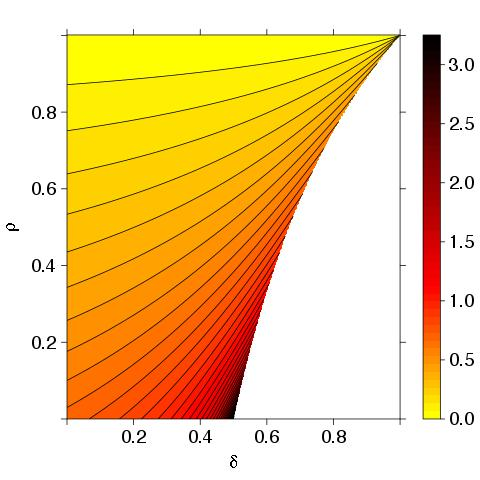
\includegraphics[width=\textwidth, height = \textwidth]{ExtremeN2.jpeg}
%\caption{N = 2}
%\label{ExtremeN5}
%\end{minipage}
%\begin{minipage}[t]{0.33\textwidth}
%\centering
%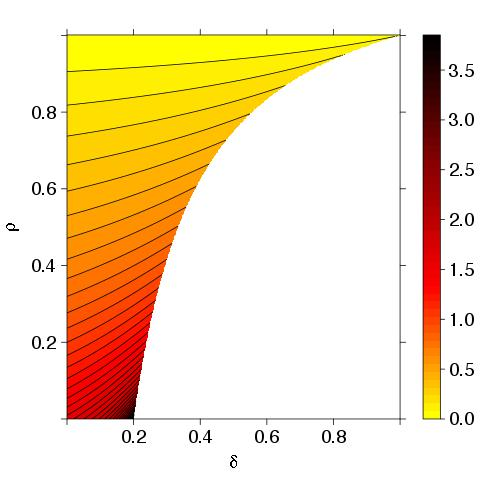
\includegraphics[width=\textwidth, height = \textwidth]{ExtremeN5.jpeg}
%\caption{N = 5}
%\label{ExtremeN10}
%\end{minipage}
%\begin{minipage}[t]{0.33\textwidth}
%\centering
%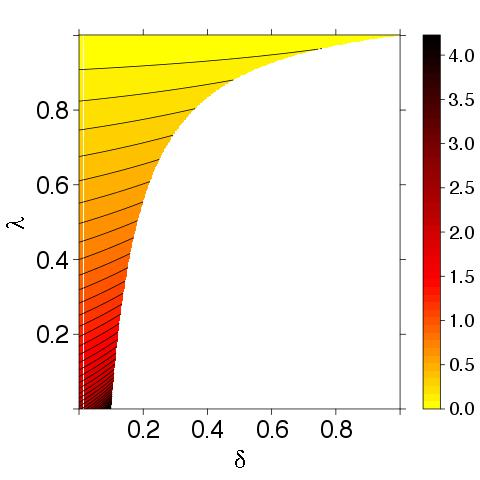
\includegraphics[width=\textwidth, height = \textwidth]{ExtremeN10.jpeg}
%\caption{N = 10}
%\label{ExtremeN30}
%\end{minipage}
%\end{figure}


\begin{figure}
        \centering
        \begin{subfigure}[b]{0.45\textwidth}
                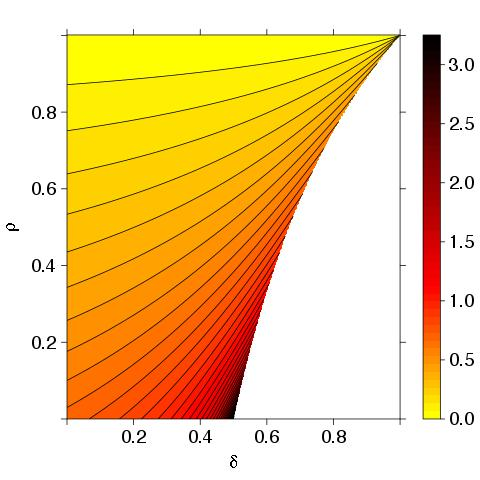
\includegraphics[width=\textwidth]{ExtremeN2.jpeg}
\caption{N = 2}	
\label{ExtremeN5}
        \end{subfigure}%
        ~ %add desired spacing between images, e. g. ~, \quad, \qquad etc.
          %(or a blank line to force the subfigure onto a new line)
%        \begin{subfigure}[b]{0.32\textwidth}
%                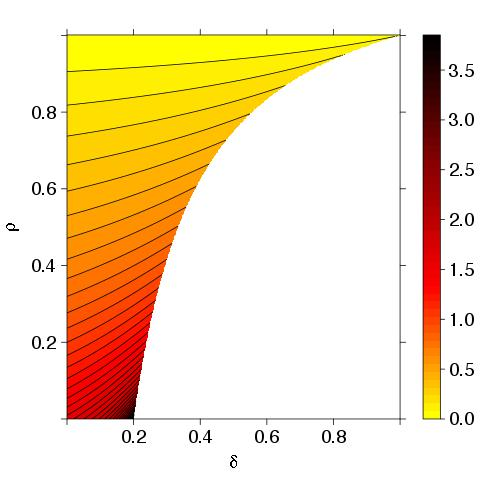
\includegraphics[width=\textwidth]{ExtremeN5.jpeg}
%\caption{N = 5}
%\label{ExtremeN10}
%        \end{subfigure}
        ~ %add desired spacing between images, e. g. ~, \quad, \qquad etc.
          %(or a blank line to force the subfigure onto a new line)
        \begin{subfigure}[b]{0.45\textwidth}
                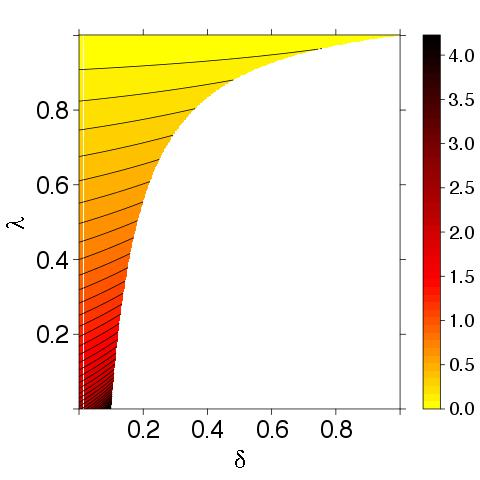
\includegraphics[width=\textwidth]{ExtremeN10.jpeg}
\caption{N = 10}
\label{ExtremeN30}
        \end{subfigure}
        \caption{ The amount of log-extremization $\log(\alpha)$ under different combinations of $N$ (the number of experts), $\delta$ (the amount of information known by one expert), and $\rho$ (the amount of information shared by any two experts).}
\end{figure}



Expression (\ref{CompoundAlpha}) is particularly convenient because it only depends on three intuitive parameters. Therefore it can be analyzed graphically. Figures \ref{ExtremeN5} and \ref{ExtremeN30} describe the amount of log-extremization $\log(\alpha)$ under different values of $\rho, \delta$, and $N$. By Observation \ref{positiveThm} the amount of extremizing is always greater or equal to 1.0. Notice that most extremization occurs when $\delta = 1/N$ and $\rho = 0$. In this case the group's information sets form a partition of the full information. Therefore as a group the experts know all the information. Such a group can re-construct $X_S$ by simply adding up their individual probit forecasts. This means that aggregation becomes voting: if the sum of the probit forecasts is above 0, the event $A$ materializes; else it does not. A similar observation has been made under the interpreted signal framework (see the example on information aggregation in \cite{hong2009interpreted}). Therefore voting can be expected to work well when the voters in the real world form a very knowledgable and diverse group of experts. 
 

Moving away from these two extreme points towards the upper left corner, where $\delta = 0.0$ and $\rho = 1.0$, decreases the amount of extremizing monotonically to $1.0$. This decrease is caused by a) reduction in the amount of information that each individual expert holds and b) increase in the amount of shared information. Therefore the more knowledgable and diverse the group of experts is, the more their average probit forecast should be extremized. Contrast this with the classical measurement error model where higher variance is typically considered negative. Under the partial information model and the interpreted signal frameworks, however, higher variance implies broader diversity among the experts and hence is considered helpful. 

From Figures \ref{ExtremeN5} and \ref{ExtremeN30} it is clear that the feasible set of $(\delta, \rho)$-values becomes smaller as $N$ increases. This limitation arises from assuming a compound symmetric overlap structure. Having many experts, each with a considerable amount of information, simply leads to unavoidable overlap in the information sets. From the domain restriction on $\rho$, it is clear that $\rho \to 1$ as $N \to \infty$. Therefore in the limit the group of experts is equivalent to a single expert. This observation clearly does not reflect the real-world. When $N = 2$, on other hand, the compound symmetric overlap is almost fully general. Therefore assuming a compound symmetric information structure can be appropriate for small numbers of experts but becomes overly restrictive as more experts enter the group. 

%\subsection{Information in the Sample Average}
%It is possible to determine the amount of information in the sample average. This is done by first computing the aggregate probability for the sample average, and then finding the amount of information that a single expert should have in order for his aggregate probability to match with the aggregate probability of the sample average. That is, if $\delta_X$ denotes the information in the sample average, then 
%\begin{align*}
%%\frac{1}{\sqrt{1-\delta_X}} &= \frac{\frac{N}{(N-1)\rho +1}}{\sqrt{1- \frac{N\delta}{(N-1)\rho +1} }} \\
%\alpha &= \frac{1}{\sqrt{1-\delta_X}} &\Leftrightarrow&& \delta_X &=1-\alpha^{-2}
%\end{align*}
%Based on these equation we notice that there is a monotonic and positive relationship between $\alpha$ and $\delta_X$. This means that the more the sample average is extremized the more information it contains, and \textit{vice versa}. This result is interesting because it allows the researcher to first use black-box models from earlier literature to determine the amount of extremization and then use this quantity to analyze the portion of information that is present in the sample average. 

%
%
%\subsection{Integrate over the prior distribution}
%
%In this section we assumed that we know how much each expert knows but have no idea how much each information each experts shares. Denote $M = \max \left\{ \frac{N\delta-1}{N-1}, 0\right\}$ and assume a uniform prior on $\rho \in [M, \delta]$. That is, let $p(\rho) = (\delta - M)^{-1}$. Then,
%\begin{align*}
%\E_\rho[\alpha] &= \E \left[\frac{\frac{\delta N}{(N-1)\rho +\delta}}{\sqrt{1- \frac{N\delta^2}{(N-1)\rho +\delta} }} \right]\\
%&= (\delta - M)^{-1}  \int_{M}^\delta \frac{\frac{\delta N}{(N-1)\rho +\delta}}{\sqrt{1- \frac{N\delta^2}{(N-1)\rho +\delta} }}   d\rho\\
%\end{align*}
%Let $z = (N-1)\rho +\delta$. Then $dz = (N-1)d\rho \Rightarrow (N-1)^{-1}dz = d\rho$   and 
%\begin{align*}
%&= \frac{1}{(N-1)(\delta - M)}  \int_{(N-1)M+\delta}^{N\delta} \frac{\frac{\delta N}{z} }{\sqrt{1- \frac{N\delta^2}{z} }}  dz\\
%&= \frac{N\delta}{(N-1)(\delta - M)} \int_{(N-1)M+\delta}^{N\delta} \frac{1}{\sqrt{z^2- N\delta^2 z }}  dz\\
%&= \frac{N\delta}{(N-1)(\delta - M)} \int_{(N-1)M+\delta}^{N\delta} \frac{1}{\sqrt{z^2- 2 \frac{N\delta^2}{2} z + \left( \frac{N\delta^2}{2} \right)^2 - \left( \frac{N\delta^2}{2} \right)^2}}  dz\\
%&= \frac{N\delta}{(N-1)(\delta - M)} \int_{(N-1)M+\delta}^{N\delta} \frac{1}{\sqrt{\left( z- \frac{N\delta^2}{2} \right)^2 - \left( \frac{N\delta^2}{2} \right)^2}}  dz
%\end{align*}
%Let $u =  z- \frac{N\delta^2}{2}$. Then $du = dz$ and 
%\begin{align*}
%&=\frac{N\delta}{(N-1)(\delta - M)} \int_{(N-1)M+\delta- \frac{N\delta^2}{2}}^{N\delta- \frac{N\delta^2}{2}} \frac{1}{\sqrt{u^2 - \left( \frac{N\delta^2}{2} \right)^2}}  du\\
%&= \frac{N\delta}{(N-1)(\delta - M)} \left\{\log \left(\sqrt{4u^2 - \delta^4N^2} + 2u \right) \right\}\bigg|_{(N-1)M+\delta- \frac{N\delta^2}{2}}^{N\delta- \frac{N\delta^2}{2}}\\
%&= \frac{N\delta}{(N-1)(\delta - M)} \left\{\log \frac{ \sqrt{4\left( N\delta- \frac{N\delta^2}{2} \right)^2 - \delta^4N^2} + 2\left(N\delta- \frac{N\delta^2}{2} \right)}{\sqrt{4\left( (N-1)M+\delta- \frac{N\delta^2}{2} \right)^2 - \delta^4N^2} + 2\left( (N-1)M+\delta- \frac{N\delta^2}{2} \right) } \right\}\\
%%&= \frac{N\delta}{(N-1)(\delta - M)} \left\{\log \frac{N \sqrt{4\delta^2 \left(1- \frac{\delta}{2} \right)^2 - \delta^4} + 2\left(N\delta- \frac{N\delta^2}{2} \right)}{\sqrt{4\left( (N-1)M+\delta- \frac{N\delta^2}{2} \right)^2 - \delta^4N^2} + 2\left( (N-1)M+\delta- \frac{N\delta^2}{2} \right) } \right\}\\
%\end{align*}
%This can be plotted on a grid of values of $\delta$ and $N$. 
%\begin{center}
%   \includegraphics{rhoIntegratedPrior.jpeg} % requires the graphicx package
%\end{center}
%Moving from the middle to the right, the extremizing stengtens as the experts know more. The less intuitive result is close to the bottom-left corner of the plot. Moving diagonally from the origin, the amount of extremizing increases until the point hits the line $\delta = 1/N$. We must keep in mind that the extermination is always relative to the given mean. If there are many experts that know, say, 0.20, then their mean is (under non-informative prior on $\rho$) much more informative than the mean of only a few experts who know the same amount. Therefore you should extremize the smaller group more. 
%
%
%If $M = 0 \Leftrightarrow \delta \leq 1/N$ , this equals to 
%\begin{align*}
%&= \frac{ N \log \left( (2-\delta+2\sqrt{1-\delta})\delta N\right)}{(N-1)} -
%\frac{N \log (\delta (2 - \delta N + 2 \sqrt{1-\delta N}))}{N-1} \\
%&= \frac{N}{N-1} \left(\log \left( (2-\delta+2\sqrt{1-\delta})\delta N\right)- \log (\delta (2 - \delta N + 2 \sqrt{1-\delta N})) \right) \\
%&= \frac{N}{N-1} \left(\log \frac{2N-\delta N+2\sqrt{1-\delta}N) }{2 - \delta N + 2 \sqrt{1-\delta N}} \right) \\
%\end{align*}
%If, on other hand, $M = \frac{N \delta -1}{N-1}$, then
%
%
%%
%%\begin{verbatim}
%%delta = 0.1
%%N = 100
%%M = max((N*delta-1)/(N-1), 0)
%%integrand <- function(x) (delta-M)^(-1)*(delta*N/ ((N-1)*x+delta)) / sqrt(1 - (delta^2*N/ ((N-1)*x+delta)))  
%%integrate(integrand, lower = M, upper = delta)
%%
%%integrand <- function(x)   (N*delta/((N-1)*(delta-M))) * 1/sqrt((x-N*delta^2/2)^2 -(N*delta^2/2)^2)
%%integrate(integrand, lower = (N-1)*M+delta, upper = N*delta)
%%
%%integrand <- function(x)   (N*delta/((N-1)*(delta-M))) * 1/sqrt(x^2 -(N*delta^2/2)^2)
%%integrate(integrand, lower = (N-1)*M+delta - N*delta^2/2, upper = N*delta-N*delta^2/2)
%%
%%
%%f = function(u, delta, N) log(sqrt(4*u^2 - delta^4*N^2)+2*u)
%%
%%get.alpha = function(delta,N){
%%	M = max((N*delta-1)/(N-1), 0)
%%	up = N*delta - N*delta^2/2
%%	low = (N-1)*M + delta - N*delta^2/2
%%	 N*delta/((N-1)*(delta-M)) *(f(up, delta, N) - f(low, delta, N))
%%}
%%
%%deltas = seq(0.01, 0.99, 0.001)
%%Ns = 2:100
%%grid = expand.grid(deltas, Ns)
%%alphas = NULL
%%
%%integrand <- function(x) (delta-M)^(-1)*(delta*N/ ((N-1)*x+delta)) / sqrt(1 - (delta^2*N/ ((N-1)*x+delta)))  
%%
%%for(i in 1:nrow(grid)){
%%	#	alphas[i] = get.alpha(grid[i,1], grid[i,2])
%%	N = grid[i,2]
%%	delta = grid[i,1]
%%	M = max((N*delta-1)/(N-1), 0)
%%	alphas[i] = integrate(integrand, lower = M, upper = delta)$value
%%}
%%
%%library(lattice)
%%col.l = c(colorRampPalette(c('skyblue', 'darkblue'))(9), colorRampPalette(c('darksalmon', 'darkred'))(11))
%%ats = c(seq(0, 1, length = 10), seq(1, max(alphas, na.rm = TRUE), length = 11))
%%ats = ats[-10]
%%levelplot(alphas~grid[,1]+grid[,2], ylab = "N (number of experts)", xlab = "delta  (amount known by one expert)", col.regions = col.l, at = ats, pretty = TRUE)
%%
%%
%%plot(alphas[grid[,2] == 10]~deltas, type = "l")
%%abline(v = 1/10)
%%
%%\end{verbatim}
%
%\subsection{Integrate over the posterior distribution}
%In this section, we investigate the amount of extremizing after integrating out $\rho$ with respect to its posterior distribution. 


%\subsection{Prior information}
%
%\section{Inverse Problem}


\section{Multinomial Outcomes}
If the target event can take upon $K > 2$ outcomes, the the white noise process must be extended to a $(K-1)$-dimensional process $\{ \boldsymbol{X}_B \}$ with each $\boldsymbol{X_B} = (X_{1,B}, X_{2,B},  \dots, X_{K-1,B})' \in \mathbb{R}^{K-1}$.  Expert $j$ observes a fixed share $\delta_j$ of the process. If the information sets of two experts $i$ and $j$ overlap, i.e. $| I_i \cap I_j| = \rho_{ij} > 0$, then the dependency between $\boldsymbol{X}_{I_i}$ and $\boldsymbol{X}_{I_j}$ is described by the cross-covariance $\text{cov}(\boldsymbol{X}_{I_i}, \boldsymbol{X}_{I_j}) = \rho_{ij} I_{K-1}$. Collect the coordinate-specific information sources into vectors $\boldsymbol{X}^{(k)} = \left(X_{k,I_1}, X_{k,I_2}, \dots, X_{k,I_N} \right)'$  for $k = 1, \dots, K-1$. This specifies the following multivariate normal distribution. 

\begin{align*}
\left(\begin{matrix} \boldsymbol{X}_S \\ \boldsymbol{X}^{(1)}\\ \vdots \\ \boldsymbol{X}^{(N)} \end{matrix}\right) &\sim \mathcal{N}_{}\left( 
 \boldsymbol{0}, \left(\begin{matrix} 
\Lambda_{11} & \Lambda_{12}\\
\Lambda_{21} & \Lambda_{22}\\
 \end{matrix}\right) 
 =
 \left(\begin{array}{c c c c | c c c c c}
  \multicolumn{4}{c|}{\multirow{4}{*}{$I_{K-1}$}} & \Sigma_{12}  & &  \multicolumn{2}{c}{\multirow{2}{*}{$\boldsymbol{0}$}}   \\ 
 & &  & & &  \Sigma_{12} && & \\ 
   &  &  &  &  \multicolumn{2}{c}{\multirow{2}{*}{$\boldsymbol{0}$}}  & \ddots&  \\ 
   &  &  &  &&& &\Sigma_{12}  \\ \hline
\Sigma_{21} & &\multicolumn{2}{c|}{\multirow{2}{*}{$\boldsymbol{0}$}}& \Sigma_{22} & & \multicolumn{2}{c}{\multirow{2}{*}{$\boldsymbol{0}$}}   \\ 
 & \Sigma_{21} & & &  & \Sigma_{22} &&  \\ 
\multicolumn{2}{c}{\multirow{2}{*}{$\boldsymbol{0}$}}& \ddots &&\multicolumn{2}{c}{\multirow{2}{*}{$\boldsymbol{0}$}}  & \ddots &  \\ 
&&  & \Sigma_{21} &  &  &&\Sigma_{22} \\ 
 \end{array}\right)\right),
\end{align*}
where notation is borrowed from (\ref{NExperts}). Let $\boldsymbol{X} = ((\boldsymbol{X}^{(2)})', \dots, (\boldsymbol{X}^{(K-1)})')'$.  If $\Lambda_{22}$ is a coherent overlap structure and $\Lambda_{22}^{-1}$ exists, then all $\boldsymbol{X}_{S} | \boldsymbol{X} \sim \mathcal{N}\left(\boldsymbol{\bar{\mu}}, \bar{\Lambda}\right)$, where
\begin{align*}
\boldsymbol{\bar{\mu}} &=  \Lambda_{12} \Lambda_{22}^{-1} \boldsymbol{X} &&  \bar{\Lambda}= (1 - \Sigma_{12} \Sigma_{22}^{-1} \Sigma_{21}) I_{K-1}
\end{align*}

\begin{figure}
        \centering
        \begin{subfigure}[b]{0.45\textwidth}
                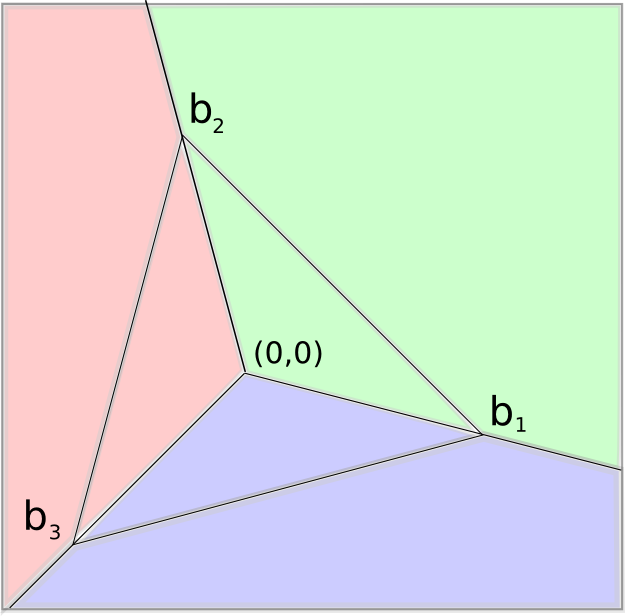
\includegraphics[width=\textwidth]{conesA.png}
\caption{Illustration of the cone partition. The cones $C_1$, $C_2$, and $C_3$ are denoted with colors red, blue, and green, respectively. }	
\label{coneA}
        \end{subfigure}%
        ~ %add desired spacing between images, e. g. ~, \quad, \qquad etc.
          %(or a blank line to force the subfigure onto a new line)
        \begin{subfigure}[b]{0.45\textwidth}
                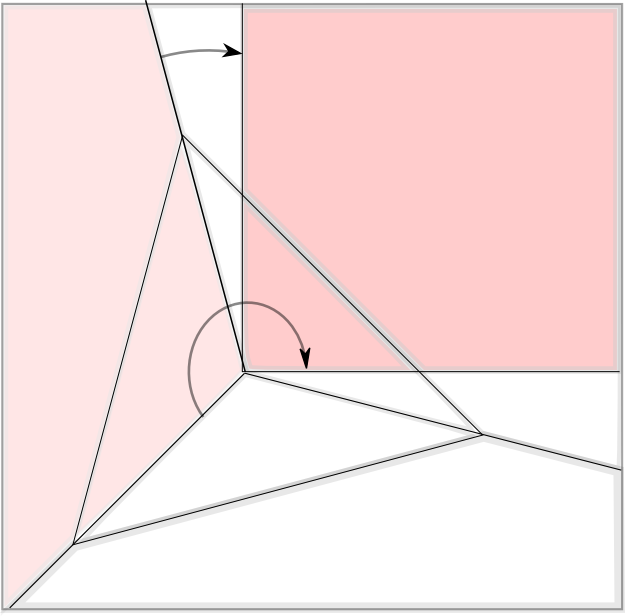
\includegraphics[width=\textwidth]{conesB.png}
\caption{Illustration of the rotation. In this example $C_1$ is rotated to the convex cone $C_e$ defined by the two standard basis vectors $\boldsymbol{e}_1$ and $\boldsymbol{e}_2$}
\label{coneB}
        \end{subfigure}
        \caption{Illustration of the model when the event can take $K = 3$ different outcomes.}
\end{figure}



The $(K-1)$-dimensional space is partitioned into $K$ cones with apexes at the origin. The target event results in the outcome $k$ if $\boldsymbol{X}_S$ is in the $k$th cone. As the different outcomes do not have a particular ordering to them, each cone must have the same shape and neighbor every other cone. This can be achieved with a regular $K$-simplex that has been centered at the origin. More specifically, if $A = \frac{1- \sqrt{K}}{K-1}$ and $B = \frac{1+A}{K}$, then the $K$ vertices of the simplex are given by 
\begin{align*}
\boldsymbol{b}_1 &= (1-B, -B, -B, \dots, -B)'\\
\boldsymbol{b}_2 &= (-B, 1-B, -B, \dots, -B)'\\
& \phantom{=}\vdots\\
\boldsymbol{b}_{K-1} &= (-B, -B, -B, \dots, 1-B)'\\
\boldsymbol{b}_{K} &= \left(A-B, A-B, \dots, A-B \right)'
\end{align*}
%http://mathoverflow.net/questions/38724/coordinates-of-vertices-of-regular-simplex
The $k$th cone $C_k$ is the convex cone defined by all vertices except the $k$th one. That is, 
\begin{align*}
C_k &= \{\boldsymbol{b}_1\theta_1 + \dots + \boldsymbol{b}_{k-1}\theta_{k-1} + \boldsymbol{b}_{k+1}\theta_{k+1} + \boldsymbol{b}_{K}\theta_{K} | \theta_1, \theta_2, \dots, \theta_K \geq 0\} 
\end{align*}
Figure \ref{coneA} illustrates the construction of cones under $K = 3$ different outcomes. The cones $C_1$, $C_2$, and $C_3$ are denoted with colors red, blue, and green, respectively. The aggregate probability for the $k$th outcome is computed by integrating over $C_k$ with respect to the conditional distribution of $\boldsymbol{X}_S$. This integration is much easier if $C_k$ is first transformed into the convex cone defined by the first $K-1$ standard basis functions. Figure \ref{coneB} illustrates the transformation for $C_1$.  Denote the standard cone with $C_e$ and let 
\begin{align*}
T_k &= \left(\begin{matrix} 
\boldsymbol{b}_1& \dots & \boldsymbol{b}_{k-1} & \boldsymbol{b}_{k+1} & \dots & \boldsymbol{b}_K
 \end{matrix}\right) ^{-1}
\end{align*}
represent the transformation matrix for $C_k$. Define the function $F(\boldsymbol{x}_0 | \boldsymbol{\mu}, \Sigma)$ of a random variable $\boldsymbol{x} \sim \mathcal{N}_N(\boldsymbol{\mu}, \Sigma)$ as the probability that all of the components of $\boldsymbol{x}$ are \textit{greater or equal} to the corresponding elements in $\boldsymbol{x}_0$. Then the aggregator is 
\begin{align}
\P(\boldsymbol{X}_S \in C_k | \boldsymbol{X}) &= \P(T_k \boldsymbol{X}_S \in C_e | \boldsymbol{X}) \nonumber\\
&= F(\boldsymbol{0} | T_k\boldsymbol{\bar{\mu}}, T_k' \bar{\Lambda}T_k) \label{MultiAggre}
\end{align}
By construction the aggregate probabilities for the $K$ outcomes sum to one. The aggregator (\ref{MultiAggre}) provides the map from a probability forecast to the corresponding probit forecast made by an expert. More specifically, the probability forecasts for the $k$th outcome made by the $j$th expert is
\begin{align*}
p_{kj}&= F(\boldsymbol{0} | T_k\boldsymbol{X}_{I_j}, (1-\delta_j)T_k'T_k)
\end{align*}
Similarly to the binary case, the expert's probability forecasts are marginally uniform over the vertices of the $K$-simplex when $\delta_j = 1$. This marginal distribution converges to the center of the simplex, i.e. the point $(1/K, 1/K, \dots, 1/K)$ as $\delta_j \to 0$. 

\section{Discussion}
This paper introduced a novel framework for analyzing subjective response data. Under this framework any response heterogeneity is assumed to arise from cognitive diversity. The mathematical tractability and real-world applicability of this model were illustrated by deriving an information theoretic aggregation rule for multiple probability forecasts. The aggregator resulted in closed-form expression for the amount of extremization that should be performed for the average probit forecast. By assuming a simplified information structure, the amount of extremization was studied graphically. This led to many insights on extremization. Given that these insights tend to align with common sense, the framework appears to be appropriate for probability aggregation.

Part of our future work is to continue developing the aggregator under the partial information framework. It is possible to place flexible priors on the unknown parameters and marginalize them with respect to their posterior distributions. This would lead to a principled aggregator that does not require any training. Instead, it could be applied directly to the data and would replace suboptimal methods such as the mean or median. As was discussed in Section \ref{extremization}, assuming a compound symmetric information structure is hardly a realistic choice. Therefore it will be necessary to develop a class of information structures that reflect the reality more closely. As it is unlikely that such a structure will lead to an aggregator with a closed-form solution, the aggregator will be provided in the form of an efficient algorithm.

Another future direction is to derive an information theoretic aggregator for subjective distributions. This is an important problem in Bayesian statistics where the analysis heavily depends on the choice of the prior distribution. Often the prior distribution is picked subjectively by the scientist who has previous experience on the problem at hand. If, however, the experiment is conducted by a group of scientists, their prior distributions must aggregated before the statistical analyses can be carried out. 
 
The partial information framework is clearly a simplification of the reality. For instance, assuming that each expert produces an optimal probability forecast given his information set may not be a realistic assumption. The experts may believe in false information, hide their true beliefs, or be biased for many other reasons. This could be incorporated in the model by introducing an error term, possibly with a mean of zero, that is applied to the experts' probit forecasts. The resulting model, which is a hybrid of the generated signal and partial information frameworks, could lead to more realistic results. This improvement, however, may require a sacrifice in mathematical convenience. 


%\bibliographystyle{plain}
\bibliographystyle{plainnat}
\bibliography{biblio}		% expects file "myrefs.bib"



\end{document}
